La vista de implementación e instalación representada en el diagrama~\ref{fig:vista-implementacion-instalacion} describe la infraestructura tecnológica que soporta la ejecución de aplicaciones dentro del entorno \GRID. En la capa de tecnología, se identifican diversos nodos que alojan instancias de Containerd, encargadas de orquestar la ejecución de contenedores que materializan las funcionalidades de la capa de aplicación. Estos nodos se encuentran interconectados con un subsistema de almacenamiento compartido, lo que garantiza la persistencia y disponibilidad de datos. La comunicación de red es gestionada mediante servicios de \NAT\ y DHCP, con mecanismos de failover que buscan la continuidad operativa. La capa de virtualización se representa con el hipervisor XCP-NG, desplegado sobre la \LAN\ del clúster, cuya conectividad está protegida por un firewall del clúster. A nivel externo, la \LAN\ \GRID\ y el \textit{firewall} \GRID\ constituyen la frontera de seguridad antes del acceso a Internet. En conjunto, la vista refleja cómo los \textit{Infrastructure Services} (almacenamiento, red, virtualización y seguridad) soportan la ejecución de aplicaciones en un entorno distribuido, robusto y seguro, alineado con la arquitectura actual del \GRID.
\begin{figure}[H]
    \centering
    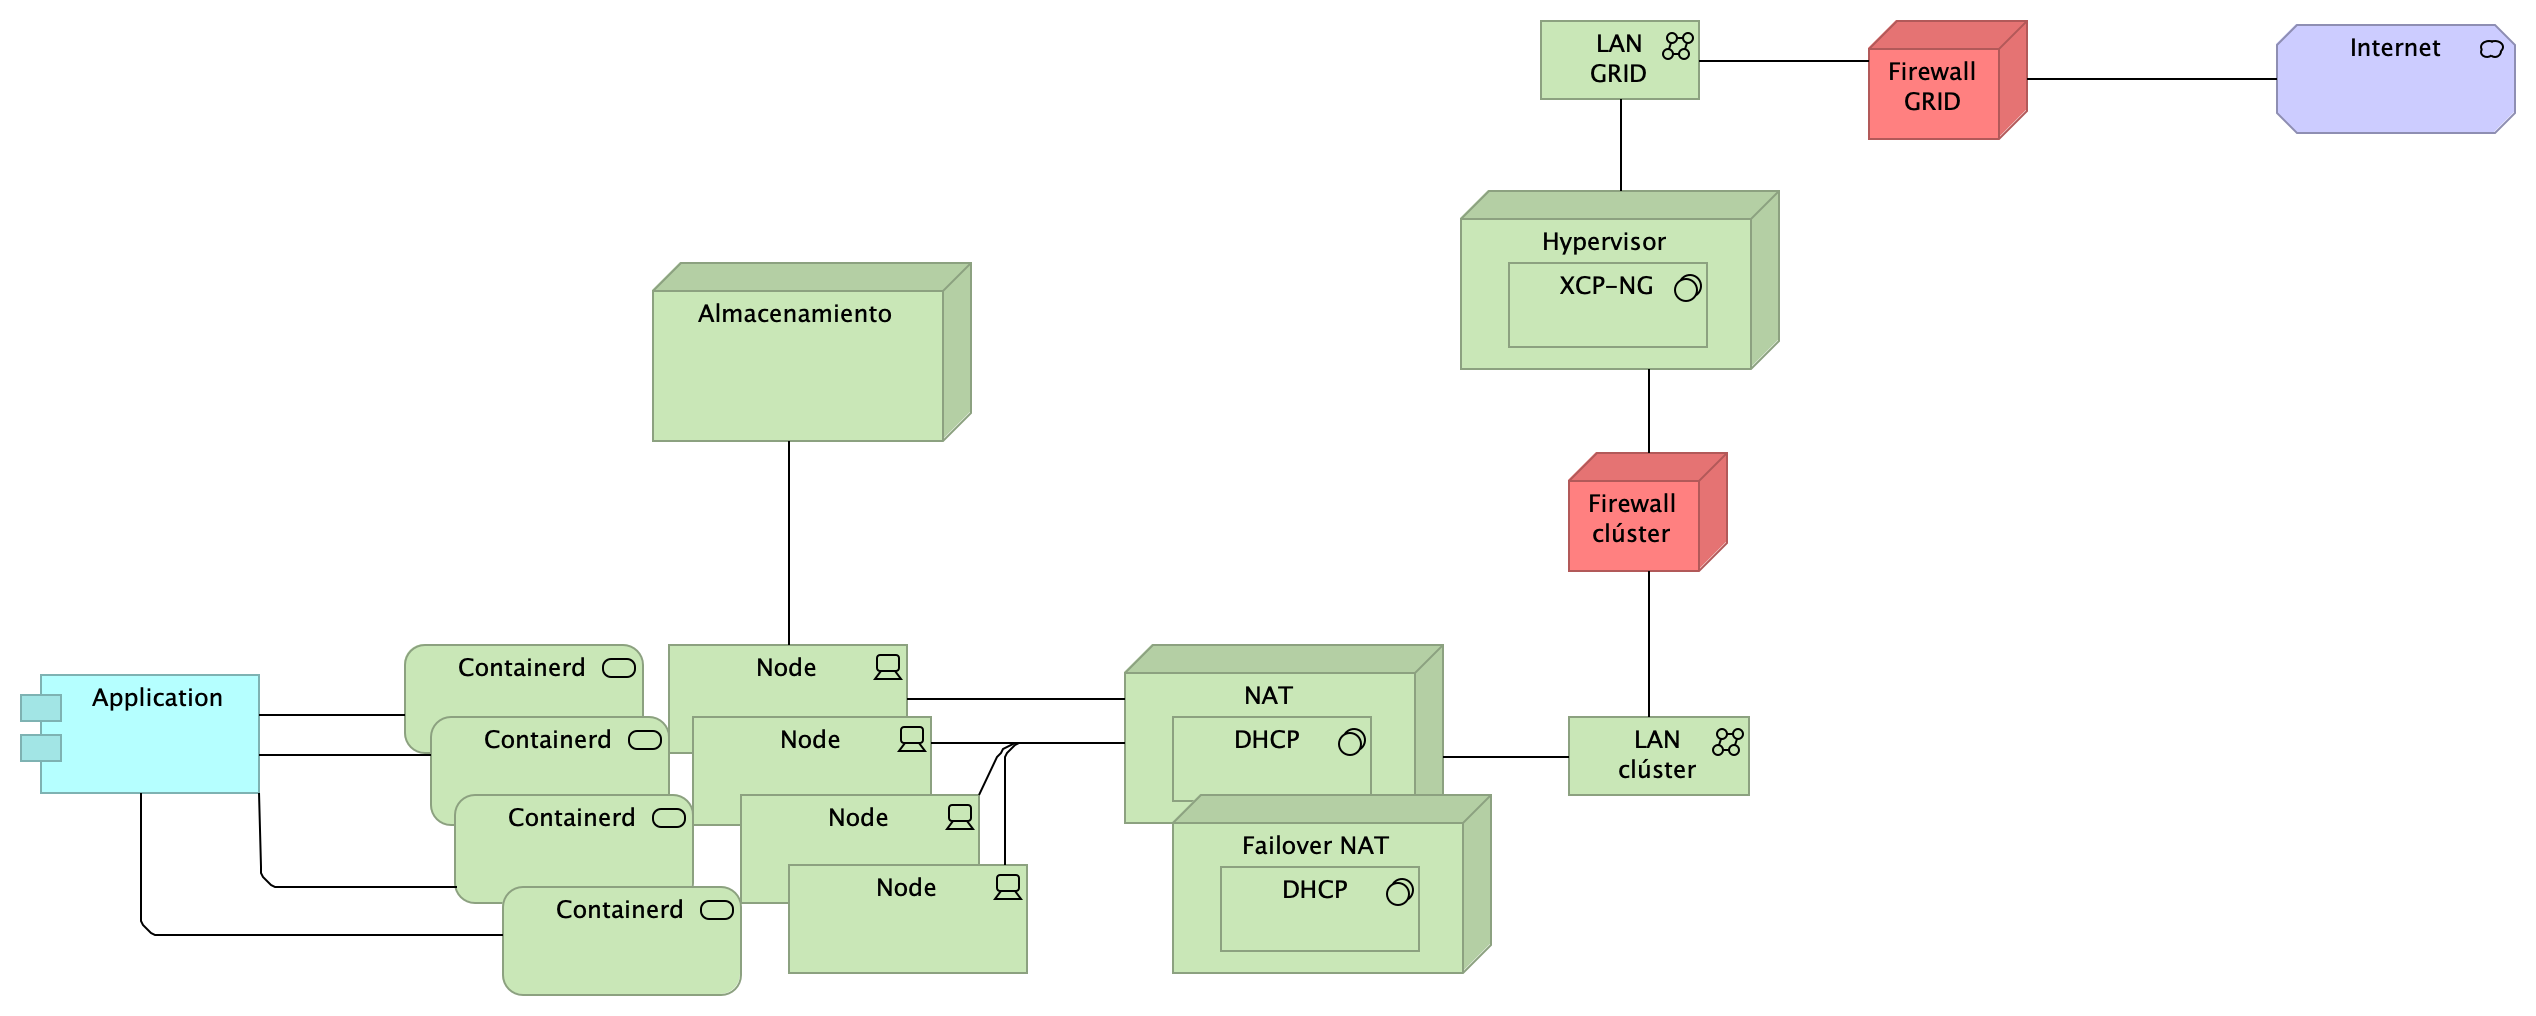
\includegraphics[width=\textwidth]{tablas-images/cp6/Implementation-and-Installation-View.png}
    \caption{Vista de Implementación e Instalación}\label{fig:vista-implementacion-instalacion}
\end{figure}
\noindent
La vista~\ref{fig:vista-informacion} representada en el diagrama de ArchiMate describe cómo se organiza y gestiona el flujo de datos y políticas que regulan el uso del \GRID. En el centro, el \textit{Data Object} Perfil de Estudiante/Investigador \GRID\ articula la relación entre el Usuario/Investigador \GRID\ y los procesos de gestión de solicitudes y ejecución. Dicho perfil se vincula con \textit{Data Objects} como los Datos de Usuario/Credenciales, los Datos de Solicitud (YAML/JSON) y los Resultados de Ejecución, los cuales proporcionan información para habilitar el acceso, desplegar contenedores y registrar salidas de los trabajos. Sobre esta base, se modelan diferentes Business Rules y Policies, entre ellas: Política de Uso, Política de Ejecución de Jobs Cortos/Interactivos, Política de Ejecución de Jobs de Alto Consumo (\HPC), Política de Ejecución en Entornos Persistentes, Política de Gestión de Errores y Política de Soporte y Reintentos Automáticos. Todas estas se encuentran interconectadas y se apoyan en parámetros técnicos como cuotas y límites de \CPU, memoria, \GPU y almacenamiento. Finalmente, la Ejecución de Job aparece como punto de materialización de dichas políticas, integrando la información contenida en formularios YAML de ejecución con las restricciones y lineamientos establecidos.
\begin{figure}[H]
    \centering
    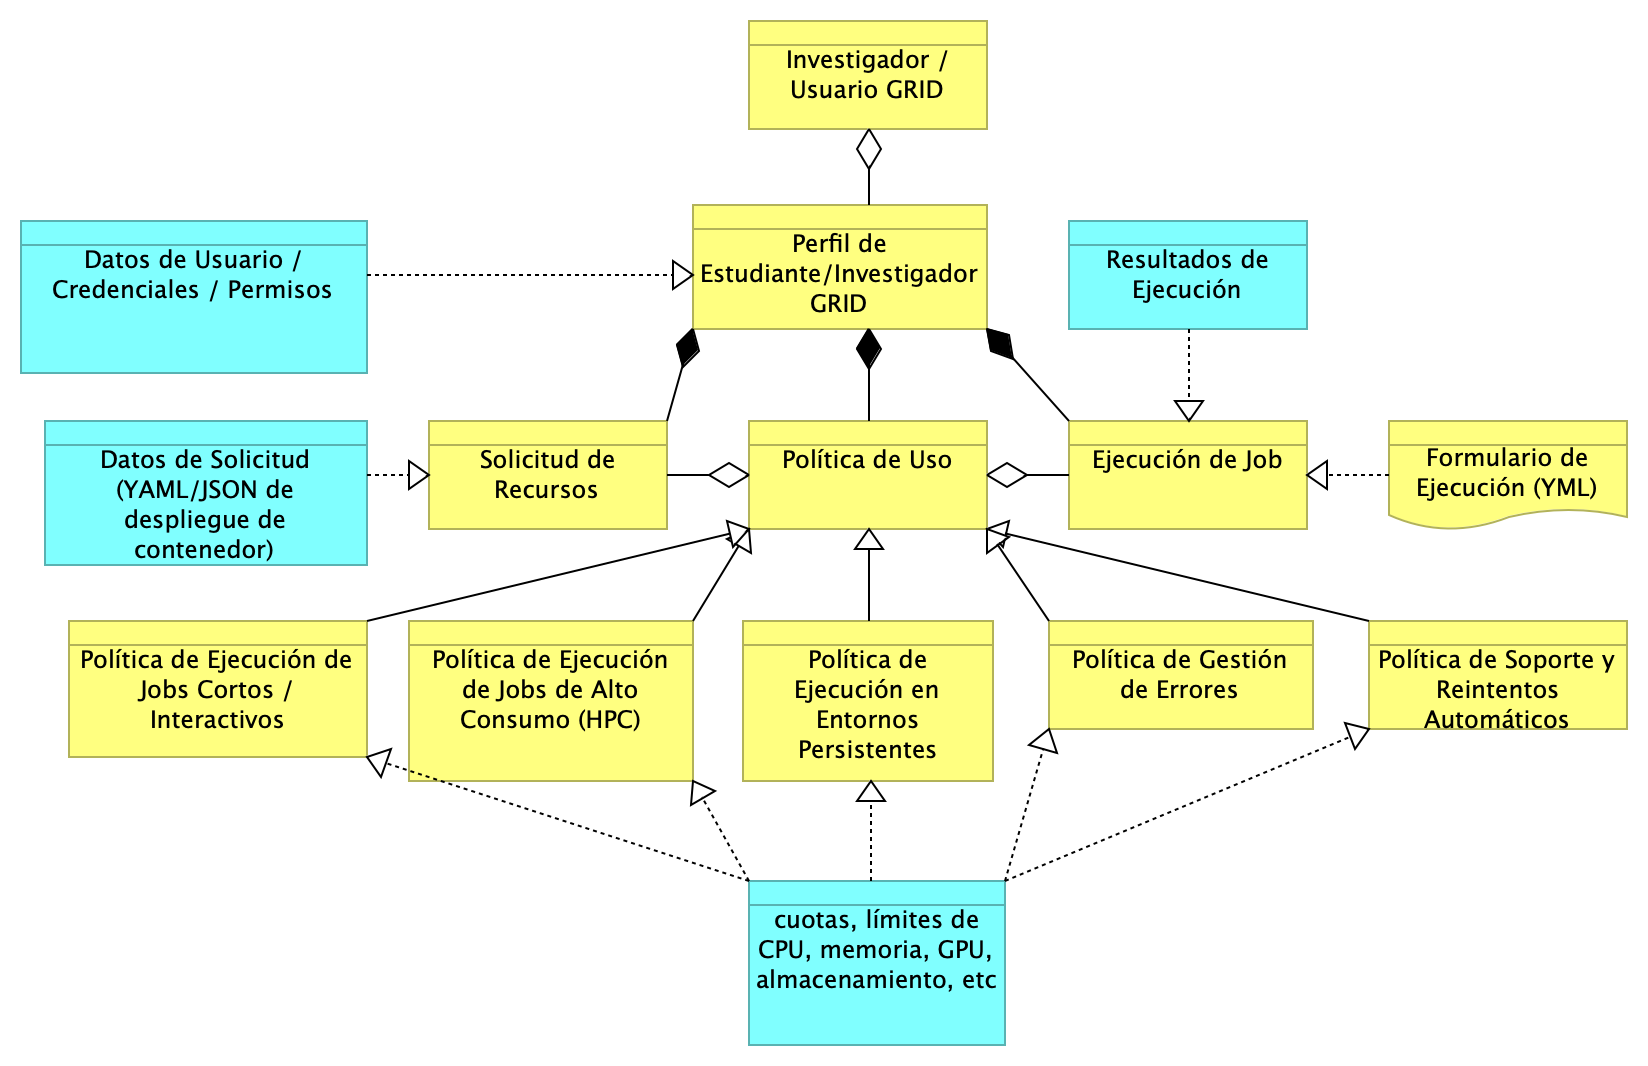
\includegraphics[width=\textwidth]{tablas-images/cp6/Information-Structure-View.png}
    \caption{Vista de Estructura de Información}\label{fig:vista-informacion}
\end{figure}